\documentclass[12pt]{article}
\setlength{\oddsidemargin}{0in}
\setlength{\evensidemargin}{0in}
\setlength{\textwidth}{6.5in}
\setlength{\parindent}{0in}
\setlength{\parskip}{\baselineskip}

\usepackage{amsmath,amsfonts,amssymb,graphicx,xcolor,mathtools}

\newcommand{\purple}[1]{{\color{purple} #1}}

%\title{Review of Newtonian Mechanics}

\begin{document}

PHYS 374 Fall 2020\hfill Worksheet 5: Coupled Oscillators\\
\\
Name: \purple{PARTIAL SOLUTION -- FINISH ON YOUR OWN!}\\
\\
Please submit as a PDF on Moodle. Include any calculations made using external tools.

\hrulefill
\\
\\
Consider two identical blocks suspended by three identical springs as shown below. All motion is horizontal. When at rest, all springs are unstretched. 
\begin{figure}[h]
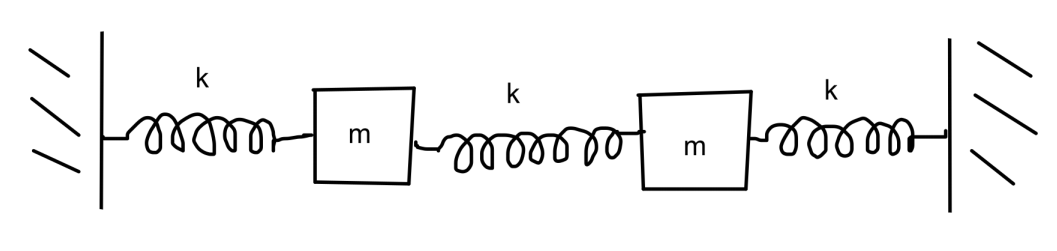
\includegraphics[width=10cm]{coupled-oscillators.png}
\centering
\end{figure}
\begin{enumerate}
\item Write down the Lagrangian for this system. How many degrees of freedom are there?

\purple{
There are two degrees of freedom. The natural choice of coordinates is $x_1$ as the position of the first block and $x_2$ as the position of the second block. It's furthermore convenient to measure $x_1$ and $x_2$ from the resting positions of the blocks so we don't have to worry about the length of the springs. Then:
$$
\mathcal{L} = 
\underbrace{
\tfrac{1}{2} m \dot{x_1}^2 + \tfrac{1}{2} m \dot{x_2}^2
}_{T}
\underbrace{
- \tfrac{1}{2} k x_1^2 - \tfrac{1}{2} k \left( x_1 - x_2 \right)^2 - \tfrac{1}{2} k x_2^2
}_{-U}
$$
The two $T$ terms are the one-dimensional kinetic energy of the blocks, and the three $U$ terms are the potential energies associated with the three springs (in order).}
\item Determine the equations of motion for this system. Notice that they are coupled so we cannot solve them directly!

\purple{
\begin{align*}
\frac{\partial \mathcal{L}}{\partial x_1} &= \frac{d}{dt} \frac{\partial \mathcal{L}}{\partial \dot{x_1}}
& &\rightarrow&
-2kx_1 + kx_2 &= m\ddot{x_1} \\
\frac{\partial \mathcal{L}}{\partial x_2} &= \frac{d}{dt} \frac{\partial \mathcal{L}}{\partial \dot{x_2}}
& &\rightarrow&
kx_1 -2kx_2 &= m\ddot{x_2}
\end{align*}
}
\item Combine the two coupled differential equations into one expression using a $2\times2$ matrix.

\purple{
$$
-\frac{k}{m}
\left[
{\begin{array}{cc}
   2 & -1\\
   -1 & 2\\
  \end{array} }
\right]
\left[
{\begin{array}{c}
   x_1\\
   x_2\\
  \end{array} }
\right] = 
\left[
{\begin{array}{c}
   \ddot{x_1}\\
   \ddot{x_2}\\
  \end{array} }
\right]
$$
}
\item Make a guess as to the form of the solution, and evaluate derivatives accordingly.

\purple{
The whole system is made of springs, so presumably the solution is some sort of oscillation. Guess:
$$
x_1(t) = A\cos \left( \omega t \right)
\quad\text{and}\quad
x_2(t) = B\cos \left( \omega t \right)
$$
Note: if $x(t) \sim \cos \left( \omega t \right)$ then $\dot{x}(0) = 0$. For initial conditions with non-zero starting velocity, we would be better off with $\cos\left( \omega t - \phi_0 \right)$ instead. But we're not worrying about initial conditions today, so we can leave off the $\phi_0$ for the sake of brevity.

Our coupled differential equations now look like:
$$
-\frac{k}{m}
\left[
{\begin{array}{cc}
   2 & -1\\
   -1 & 2\\
  \end{array} }
\right]
\left[
{\begin{array}{c}
   A\\
   B\\
  \end{array} }
\right]
\cos \left( \omega t \right)
= 
- \omega^2
\left[
{\begin{array}{c}
   A\\
   B\\
  \end{array} }
\right]
\cos \left( \omega t \right)
$$
Or simply:
$$
\frac{k}{m}
\left[
{\begin{array}{cc}
   2 & -1\\
   -1 & 2\\
  \end{array} }
\right]
\left[
{\begin{array}{c}
   A\\
   B\\
  \end{array} }
\right]
= 
\omega^2
\left[
{\begin{array}{c}
   A\\
   B\\
  \end{array} }
\right]
$$
}
\item Find the eigenvalues and eigenvectors. Hint: the eigenvalues of the expression below
are $\lambda=1$ and $\lambda = 3$.

$$
\left[
{\begin{array}{cc}
   2 & -1\\
   -1 & 2\\
  \end{array} }
\right]
\left[
{\begin{array}{c}
   x\\
   y\\
  \end{array} }
\right]
 = 
 \lambda\left[
{\begin{array}{c}
   x\\
   y\\
  \end{array} }
\right]
$$

\purple{
Lining up our expression with the hint above, we can see that $\lambda = \frac{\omega^2 m}{k}$. Or, more usefully, $\omega = \sqrt{\frac{\lambda k}{m}}$. Recall that $\omega$ is our frequency of oscillation. That means this system has two resonant frequencies: $\omega = \sqrt{\frac{k}{m}}$ and $\omega = \sqrt{\frac{3k}{m}}$. For comparison, the resonant frequency of a simple mass on a spring is $\omega = \sqrt{\frac{k}{m}}$.

Once we know the eigenvalues, we can crunch out the eigenvectors. Plugging $\omega = \sqrt{\frac{k}{m}}$ back into our expression and cancelling out a few terms, we get:
$$
\left[
{\begin{array}{cc}
   2 & -1\\
   -1 & 2\\
  \end{array} }
\right]
\left[
{\begin{array}{c}
   A\\
   B\\
  \end{array} }
\right]
 = 
 \left[
{\begin{array}{c}
   A\\
   B\\
  \end{array} }
\right]
$$
This can be solved for $A = B$.

Likewise, the following expression (using $\omega = \sqrt{\frac{3k}{m}}$) can be solved for $A = -B$:
$$
\left[
{\begin{array}{cc}
   2 & -1\\
   -1 & 2\\
  \end{array} }
\right]
\left[
{\begin{array}{c}
   A\\
   B\\
  \end{array} }
\right]
 = 
 3
 \left[
{\begin{array}{c}
   A\\
   B\\
  \end{array} }
\right]
$$
}
\item Explain (using words) the two resonant modes of this system.

\purple{
Recall that we guessed a solution of the form:
$$
x_1(t) = A\cos \left( \omega t \right)
\quad\text{and}\quad
x_2(t) = B\cos \left( \omega t \right)
$$
The first solution we found had frequency $\omega = \sqrt{\frac{k}{m}}$ and $A = B$. Since $A = B$, the two masses move in sync with one another. The distance between them is always the same. That means the middle spring moves to the left and right, but is never stretched or compressed. Essentially, the masses oscillate independently, each behaving as if the middle spring isn't even there. Appropriately enough, the oscillation frequency is $\sqrt{\frac{k}{m}}$, the frequency of a simple mass on a spring. 

\textbf{Explain the second mode yourself! What does the movement look like? What is the frequency of that movement? Is there a way to conceptualize the problem so the movement lines up nicely with the frequency?}
}

\end{enumerate}
\end{document}